\documentclass[conference]{IEEEtran}
\IEEEoverridecommandlockouts
\usepackage{cite}
\usepackage{amsmath,amssymb,amsfonts}
\usepackage{graphicx}
\usepackage{textcomp}
\usepackage{xcolor}
\usepackage{booktabs}
\usepackage{multirow}
\usepackage{hyperref}
\usepackage{balance}

\graphicspath{{../results/}}

\title{WASP Suite: Workload Analysis for Scalable Processors}

\author{%
\IEEEauthorblockN{Shrinithi Andal (MS2025017)}
\IEEEauthorblockA{Department of Computer Science and Engineering\\
International Institute of Information Technology, Bangalore\\
Email: shrinithi.andal@iiitb.ac.in}
\and
\IEEEauthorblockN{Shikhar Mutta (MT2025114)}
\IEEEauthorblockA{Department of Computer Science and Engineering\\
International Institute of Information Technology, Bangalore\\
Email: shikhar.mutta@iiitb.ac.in}
}

\begin{document}
\maketitle

%─────────────────────────────────────────────────────────────────────────────
\begin{abstract}
Modern multicore processors promise linear performance gains as core count
increases, yet real applications frequently exhibit degraded or irregular
performance when parallelism grows beyond a certain point.  The root causes
are often poorly understood because most benchmarking tools report a single
aggregate metric that obscures where contention, synchronization, or
resource saturation actually arise.

This paper presents the Workload Analysis for Scalable Processors (WASP)
framework, a purpose-built C tool for systematically measuring how four
representative workload classes --- arithmetic-intensive (CPU), memory-intensive,
storage I/O, and mixed concurrent --- respond to changes in core count and load
intensity.  WASP records per-operation latency using high-resolution
monotonic timers, collects hardware performance counters through the Linux
\texttt{perf\_event\_open()} interface, and aggregates results across a
controlled grid of 4 core-count levels, 3 intensity levels, and 5 repetitions
per cell (240 runs total).

Measured results show that mean per-operation latency for the I/O workload
rises from 17.4~\textmu{}s at one active core to 64.5~\textmu{}s at eight cores --- a
3.7$\times$ degradation --- while CPU arithmetic latency increases only 1.4$\times$
over the same range.  Mixed workloads exhibit the steepest growth (up to
9.7$\times$ slowdown over the single-core baseline).  Hardware counter data
reveals that this degradation is driven by a combination of increased
context-switch overhead, shared cache contention, and I/O queue saturation,
all of which scale faster than the compute demand itself.
\end{abstract}

\begin{IEEEkeywords}
Multicore Performance, Benchmarking, Linux perf, Scheduling Analysis,
Cache Contention, I/O Scalability, Workload Characterization
\end{IEEEkeywords}

%─────────────────────────────────────────────────────────────────────────────
\section{Introduction}
\label{sec:intro}

A fundamental challenge in multicore systems is understanding why simply
adding more cores does not always deliver proportional performance improvement.
When a single-threaded program is parallelized across four or eight cores,
naive intuition suggests that throughput should multiply accordingly.  In
practice, the operating system scheduler, shared hardware resources (caches,
memory buses, I/O controllers), and synchronization primitives all introduce
costs that grow with concurrency and can easily overwhelm the computational
benefit of parallelism.

Identifying \emph{which} of these costs dominates for a given workload type
is non-trivial.  An arithmetic-heavy workload may scale well because each
core processes an independent stream of floating-point operations with little
resource sharing.  A storage-I/O workload, by contrast, must serialize
\texttt{fsync} operations through a kernel I/O stack and block-device queue
that is not designed for high-concurrency random access.  A mixed workload
combining CPU and memory pressure exposes a third failure mode: cache-line
contention and DRAM bandwidth saturation that are invisible in either pure
workload type alone.

There is a clear need for an integrated measurement framework that:
\begin{enumerate}
  \item Runs controlled experiments across multiple workload types, intensity
        levels, and core-count configurations in a single pipeline.
  \item Records timing at the individual operation level to separate the cost
        of computation from the cost of scheduling and synchronization.
  \item Instruments hardware performance counters alongside timing so that
        observed latency changes can be attributed to specific microarchitectural
        causes such as cache misses, IPC variation, and context-switch frequency.
  \item Reports results in a structured dataset that enables comparison across
        workload classes using a common normalized metric.
\end{enumerate}

This paper presents WASP (Workload Analysis for Scalable Processors), a
framework that addresses all four requirements.  The system is implemented in
C, runs on commodity Linux hardware, and generates both raw CSV data and
graphs for analysis.  We describe the design and implementation of WASP,
explain how results are interpreted, and report findings from a 240-run
evaluation on an Intel Core Ultra 7 155U system.

The primary contributions of this work are:
\begin{itemize}
  \item A modular C benchmarking framework for CPU, memory, I/O, and mixed
        workloads with configurable core count, intensity, and measurement
        duration.
  \item Integration with Linux \texttt{perf\_event\_open()} to collect
        per-process hardware counters without disrupting workload execution.
  \item A normalized slowdown metric that enables fair comparison across
        workload types with inherently different latency scales.
  \item A detailed empirical analysis of why latency grows with core
        count, grounded in both timing data and hardware counter evidence.
\end{itemize}

The rest of this paper is organized as follows.
Section~\ref{sec:related} surveys related work.
Section~\ref{sec:design} describes the system design.
Section~\ref{sec:perf} explains how Linux \texttt{perf} is integrated.
Section~\ref{sec:setup} describes the experimental setup.
Section~\ref{sec:results} presents results.
Section~\ref{sec:whyworse} explains why latency degrades with higher core counts.
Section~\ref{sec:discussion} discusses implications.
Section~\ref{sec:conclusion} concludes.

%─────────────────────────────────────────────────────────────────────────────
\section{Related Work}
\label{sec:related}

Understanding multicore performance limits has been a research topic since
the early days of chip multiprocessors.  Amdahl's law~\cite{gregg2020}
provides a theoretical bound on parallel speedup, but real workloads are
constrained by factors the model ignores---memory latency, I/O contention,
OS scheduler overhead, and hardware resource sharing.

LMbench~\cite{lmbench} measures isolated system primitives such as context
switch cost, memory latency, and pipe throughput.  While informative for
individual system calls, it does not run multi-workload experiments under
varying concurrency levels.  SPEC CPU~\cite{spec} evaluates processor
throughput on standardized application kernels but does not expose per-core
scaling behavior or hardware counter breakdowns.

Linux \texttt{perf}~\cite{weaver2013} is the standard kernel interface for
hardware performance counter collection.  Tools such as \texttt{perf stat}
provide per-process counter summaries, but they are designed for post-hoc
analysis of individual programs.  WASP instead uses the
\texttt{perf\_event\_open()} system call directly inside the orchestrator
to collect counters in synchrony with controlled benchmark phases.

\begin{table}[htbp]
\caption{Comparison of Benchmarking Approaches}
\label{tab:comparison}
\centering
\begin{tabular}{lcccc}
\toprule
\textbf{Feature} & \textbf{LMbench} & \textbf{SPEC} & \textbf{Phoronix} & \textbf{WASP} \\
\midrule
Multiple workload types  & partial    & --         & \checkmark & \checkmark \\
Variable core count      & --         & --         & limited    & \checkmark \\
Hardware counters        & --         & \checkmark & \checkmark & \checkmark \\
Per-operation timing     & partial    & --         & --         & \checkmark \\
Normalized slowdown      & --         & --         & --         & \checkmark \\
\bottomrule
\end{tabular}
\end{table}

%─────────────────────────────────────────────────────────────────────────────
\section{System Design}
\label{sec:design}

\subsection{Architecture}

WASP consists of three compiled executables and one analysis script:
\begin{itemize}
  \item \textbf{load\_generator}: spawns actual workload threads for a given
        type and intensity, writes measured operation counts and elapsed time
        to a metrics file on completion.
  \item \textbf{benchmark}: the orchestrator.  It iterates over the parameter
        grid, forks one \texttt{load\_generator} process per active core,
        assigns each process a deterministic CPU core, opens per-PID
        \texttt{perf} sessions, and aggregates results into the CSV.
  \item \textbf{analysis}: reads the CSV and prints per-workload summaries,
        scaling tables, and slowdown statistics to standard output.
\end{itemize}

\subsection{Workload Generators}

Each workload type exercises a distinct hardware resource path:

\textbf{CPU workload.} Each worker thread runs a tight loop of floating-point
arithmetic.  Operations are independent and incur no memory or I/O cost beyond
the instruction cache.  Latency is reported in microseconds per operation
(\textmu{}s/op).

\textbf{Memory workload.} Each thread performs strided reads and writes over a
working set whose size scales with intensity.  At low intensity the working set
fits in the last-level cache; at high intensity it spills to DRAM.  Latency
is reported as time per memory access (\textmu{}s/access).

\textbf{I/O workload.} Each thread repeatedly executes a
\texttt{write}$\rightarrow$\texttt{fsync}$\rightarrow$\texttt{read}
cycle on a temporary file.  \texttt{fsync} forces the kernel to flush dirty
pages to storage before returning, making it the dominant cost.  Latency is
reported as time per I/O transaction cycle (\textmu{}s/cycle).

\textbf{Mixed workload.} Two thread groups run concurrently: one performing
CPU arithmetic and one performing memory accesses, simulating a process with
both compute-intensive and data-intensive phases.  Latency is reported as time
per combined operation unit (\textmu{}s/mixed-op).

\subsection{Measurement Methodology}

\textbf{Phase structure.} Each run includes a warmup phase to bring caches to
steady state, followed by a 5-second measurement phase.  Only the measurement
phase contributes to reported latency.

\textbf{Deterministic core placement.} The orchestrator assigns each worker
process to a specific CPU core using \texttt{sched\_setaffinity()}, with
workers placed on cores 0, 1, 2,~\ldots{} in order.

\textbf{Operation timing.} Each worker uses \texttt{clock\_gettime(CLOCK\_MONOTONIC)}
to record wall-clock time for a fixed batch of operations.  The orchestrator
aggregates counts and nanoseconds from all child workers and computes:
\begin{align}
L_{\text{cpu}}  &= \frac{\sum T_{\text{op}}}{\sum N_{\text{op}}}
                && [\mu\text{s/op}] \\
L_{\text{mem}}  &= \frac{\sum T_{\text{access}}}{\sum N_{\text{access}}}
                && [\mu\text{s/access}] \\
L_{\text{io}}   &= \frac{\sum T_{\text{cycle}}}{N_{\text{cycle}}}
                && [\mu\text{s/cycle}] \\
L_{\text{mix}}  &= \frac{\sum T_{\text{mix}}}{\sum N_{\text{mix}}}
                && [\mu\text{s/mixed\text{-}op}]
\end{align}

\textbf{Normalized slowdown.} Because different workloads have different
absolute latency scales, a normalized slowdown scalar is defined as:
\begin{equation}
S = \frac{L_{\text{loaded}}}{L_{\text{baseline}}},\quad
L_{\text{baseline}} = L(\text{cores}=1,\;\text{intensity}=25\%)
\label{eq:slowdown}
\end{equation}
A value of $S=1$ means the workload performs identically to the single-core
low-intensity baseline; values above 1 indicate degradation.

%─────────────────────────────────────────────────────────────────────────────
\section{Integration of Linux Perf}
\label{sec:perf}

\subsection{Why Hardware Counters Are Needed}

Timing measurements alone reveal \emph{that} latency has increased but not
\emph{why}.  A workload that slows down as core count rises could be limited
by CPU execution throughput, by cache miss penalties, by memory bandwidth
saturation, or by kernel scheduler overhead.  Each root cause requires a
different remedy, so identifying it is essential.

Linux exposes hardware performance monitoring units through the
\texttt{perf\_event\_open()} system call.  WASP uses this interface to
collect the following counters per worker process:
\begin{itemize}
  \item \textbf{Cycles and instructions}: used to compute Instructions Per
        Cycle (IPC).  Low IPC indicates pipeline stalls.
  \item \textbf{Cache references and cache misses}: the miss rate reveals
        whether the workload's working set fits in the shared last-level cache.
  \item \textbf{Branch instructions and misses}: high branch miss rates cause
        the processor to discard speculatively executed instructions.
  \item \textbf{Context switches}: each switch forces register-state save and
        restore and can invalidate TLB entries.
  \item \textbf{CPU migrations}: rescheduling to a different core causes a
        cold-cache penalty in that core's private L1/L2 caches.
  \item \textbf{Page faults}: indicate memory allocation activity during the
        measurement window.
\end{itemize}

\subsection{Implementation Details}

The \texttt{perf\_event\_open()} call accepts a \texttt{perf\_event\_attr}
struct, a target PID, and returns a file descriptor.  WASP passes the PID of
each worker process so that only events from that worker are counted.  The
\texttt{inherit=1} flag propagates the perf session to any child threads,
ensuring that multi-threaded workloads are fully captured.

The orchestrator follows this sequence:
\begin{enumerate}
  \item Fork each worker process.
  \item Call \texttt{perf\_event\_open()} for each counter and each worker PID.
  \item Signal workers to begin the measurement phase.
  \item Workers execute operations for the configured duration (5~seconds).
  \item Call \texttt{ioctl(PERF\_EVENT\_IOC\_DISABLE)} to freeze all counter
        values at measurement end.
  \item Read counter values from each file descriptor.
  \item Read operation counts and elapsed times written by the workers, then
        aggregate into one CSV row per run.
\end{enumerate}

%─────────────────────────────────────────────────────────────────────────────
\section{Experimental Setup}
\label{sec:setup}

All experiments were conducted on:
\begin{itemize}
  \item Processor: Intel Core Ultra 7 155U (12 cores, hybrid P+E architecture).
  \item OS: Ubuntu Linux, kernel 6.14.0-37-generic.
  \item Storage: NVMe SSD (for I/O workload).
  \item RAM: 16~GB LPDDR5.
\end{itemize}

The benchmark grid covers workload types (CPU, memory, I/O, mixed) $\times$
intensity levels (25\%, 50\%, 75\%) $\times$ active core counts (1, 2, 4, 8)
$\times$ 5 repetitions, for a total of 240 runs.  Each measurement phase runs
for 5 seconds.

%─────────────────────────────────────────────────────────────────────────────
\section{Results}
\label{sec:results}

\subsection{Aggregate Summary}

Table~\ref{tab:summary} reports per-workload statistics averaged across all
core counts and intensity levels (60 runs per workload type).

\begin{table*}[t]
\caption{Summary of Mean Latency, Throughput, and Normalized Slowdown (240 Runs)}
\label{tab:summary}
\centering
\footnotesize
\setlength{\tabcolsep}{4pt}
\begin{tabular}{llcccc}
\toprule
Workload & Latency unit & Mean latency & Latency range & Mean throughput & Mean slowdown $S$ \\
\midrule
CPU    & \textmu{}s/op        & 0.0723 & 0.056--0.082 & 14.11M ops/s      & 1.274 \\
Memory & \textmu{}s/access    & 0.0169 & 0.016--0.020 & 59.14M access/s   & 0.993 \\
I/O    & \textmu{}s/cycle     & 28.14  & 8.7--96.7    & 5051~MB/s         & 2.831 \\
Mixed  & \textmu{}s/mixed-op  & 0.0829 & 0.017--0.200 & 21.21M mixed-op/s & 4.182 \\
\bottomrule
\end{tabular}
\end{table*}

The mixed workload mean slowdown of 4.18 and I/O slowdown of 2.83 stand out
because they include both low-core and high-core runs; individual high-core
cells show much higher values.

\subsection{Scaling with Active Cores}

Table~\ref{tab:corelat} shows how mean latency changes from 1 to 8 cores.

\begin{table}[htbp]
\caption{Mean Latency by Active Core Count}
\label{tab:corelat}
\centering
\begin{tabular}{lcccc}
\toprule
Workload & 1 core & 2 cores & 4 cores & 8 cores \\
\midrule
CPU (\textmu{}s/op)        & 0.0563 & 0.0797 & 0.0811 & 0.0719 \\
Memory (\textmu{}s/access) & 0.0166 & 0.0167 & 0.0168 & 0.0180 \\
I/O (\textmu{}s/cycle)     & 17.43  & 23.70  & 29.97  & 64.52  \\
Mixed (\textmu{}s/mixed-op)& 0.0194 & 0.0441 & 0.0838 & 0.1837 \\
\bottomrule
\end{tabular}
\end{table}

I/O latency grows 3.7$\times$ from 1 to 8 cores; mixed latency grows 9.5$\times$.
Memory is the most stable at only a 9\% rise.  CPU exhibits a non-monotonic
pattern explained in Section~\ref{sec:whyworse}.

\begin{figure}[htbp]
\centerline{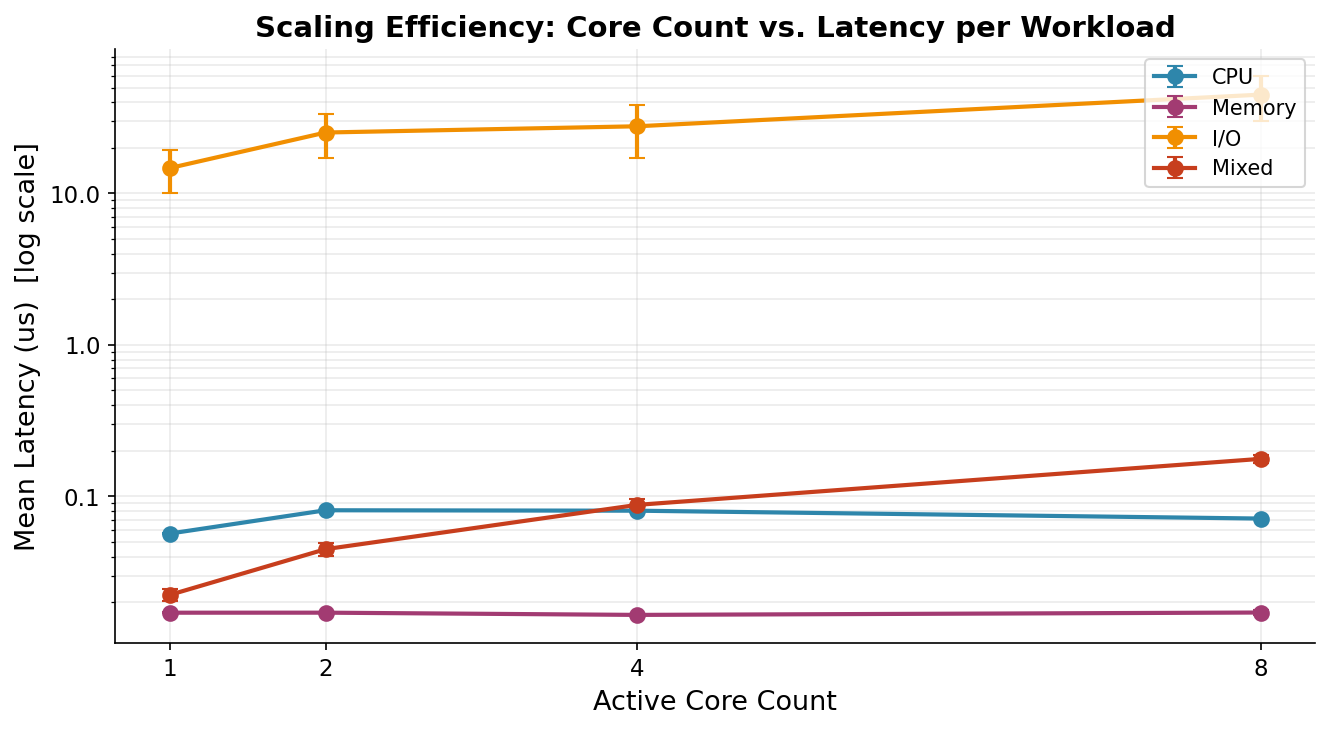
\includegraphics[width=0.98\linewidth]{scaling_efficiency.png}}
\caption{Mean latency versus active core count for each workload type (log scale).}
\label{fig:scale}
\end{figure}

\subsection{Effect of Intensity}

\begin{table}[htbp]
\caption{Mean Latency by Intensity Level}
\label{tab:intlat}
\centering
\begin{tabular}{lccc}
\toprule
Workload & 25\% & 50\% & 75\% \\
\midrule
CPU (\textmu{}s/op)        & 0.0723 & 0.0724 & 0.0721 \\
Memory (\textmu{}s/access) & 0.0170 & 0.0168 & 0.0170 \\
I/O (\textmu{}s/cycle)     & 20.11  & 26.44  & 37.87  \\
Mixed (\textmu{}s/mixed-op)& 0.0748 & 0.0800 & 0.0941 \\
\bottomrule
\end{tabular}
\end{table}

CPU and memory latency are essentially flat across intensity levels.  I/O
latency nearly doubles from 25\% to 75\% intensity because larger write
buffers take longer to flush through the kernel's block layer and NVMe
controller.

\begin{figure}[htbp]
\centerline{
\includegraphics[width=0.98\linewidth]{latency_vs_intensity.png}}
\caption{Latency versus intensity at each core-count level.  CPU and memory
are intensity-insensitive; I/O latency grows with intensity.}
\label{fig:latint}
\end{figure}

\begin{figure}[htbp]
\centerline{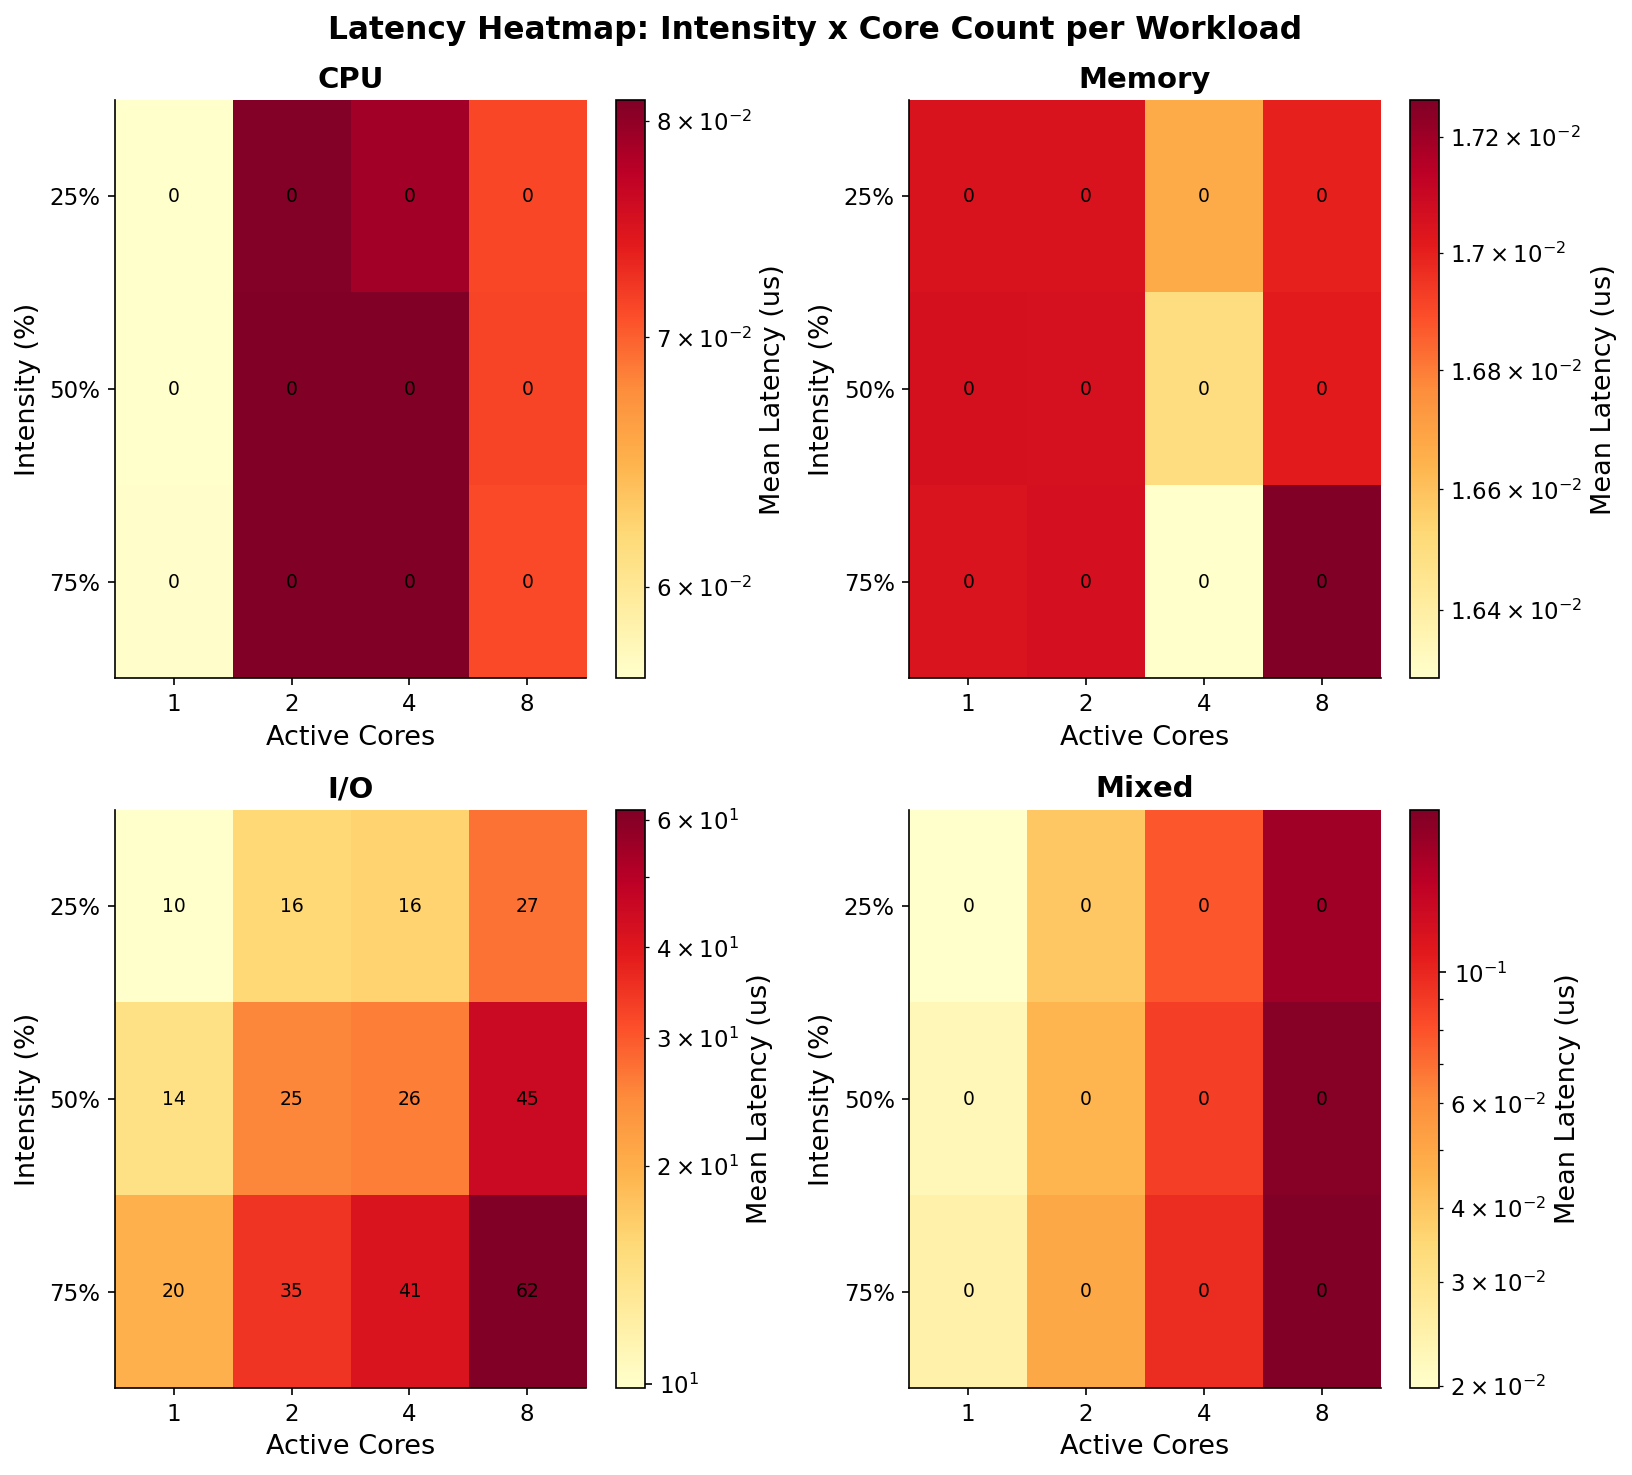
\includegraphics[width=0.98\linewidth]{latency_heatmap.png}}
\caption{Latency heatmap: mean latency as a function of intensity (rows) and
core count (columns) for each workload type.}
\label{fig:heat}
\end{figure}

\subsection{Hardware Counter Evidence}

\begin{table}[htbp]
\caption{Mean Hardware Counter Values by Workload}
\label{tab:perfmeans}
\centering
\begin{tabular}{lccc}
\toprule
Workload & IPC & Cache miss rate & Context switches \\
\midrule
CPU    & 1.787 & 0.263 & 45.0  \\
Memory & 0.863 & 0.520 & 52.1  \\
I/O    & 1.673 & 0.266 & 372.7 \\
Mixed  & 1.288 & 0.559 & 853.3 \\
\bottomrule
\end{tabular}
\end{table}

The IPC for memory (0.863) is substantially lower than for CPU (1.787),
indicating the processor stalls on memory fetches.  Cache miss rates for memory
and mixed are double those of CPU and I/O, confirming cache capacity pressure.
Context-switch counts for I/O and mixed are 8--19$\times$ higher than for CPU,
directly reflecting blocking system-call activity.

Taken together, these counters let the timing results be interpreted rather
than merely observed.  A low IPC means the core is not retiring useful
instructions quickly, while a high cache-miss rate means the core is waiting
on data that is no longer in the local or shared cache hierarchy.  When those
two signals appear alongside a large jump in context switches, the slowdown is
no longer ambiguous: the workload is spending more time waiting for the
operating system or memory subsystem than doing useful work.  That is why the
memory workload remains relatively stable while I/O and mixed workloads grow
quickly under the same core-count increase.

\begin{figure}[htbp]
\centerline{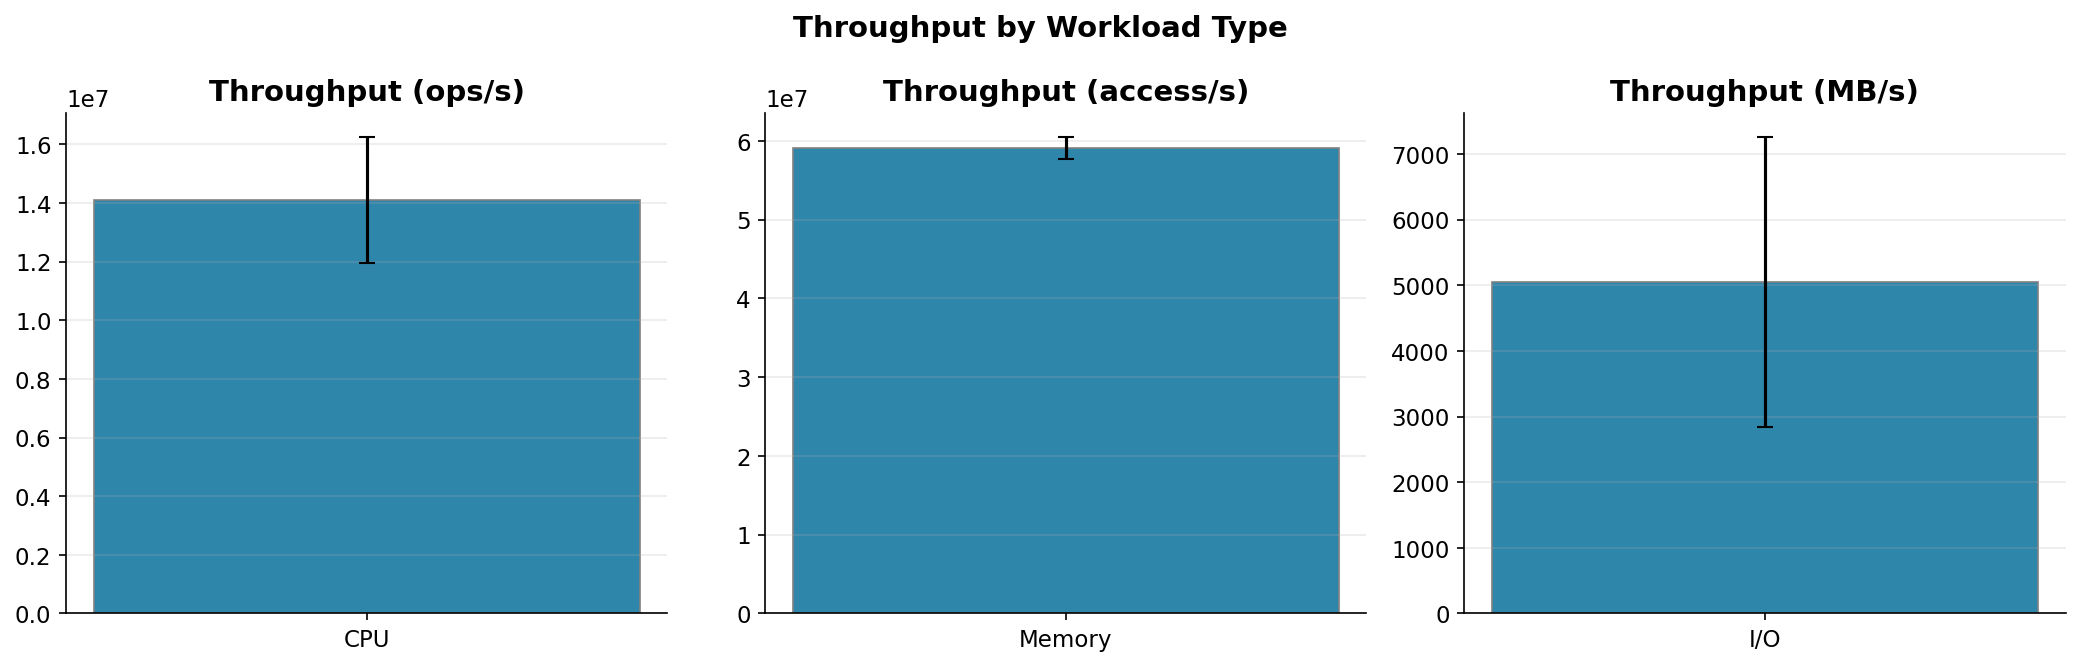
\includegraphics[width=0.98\linewidth]{throughput_by_workload.png}}
\caption{Mean throughput per workload in workload-appropriate units.}
\label{fig:thr}
\end{figure}

\begin{figure}[htbp]
\centerline{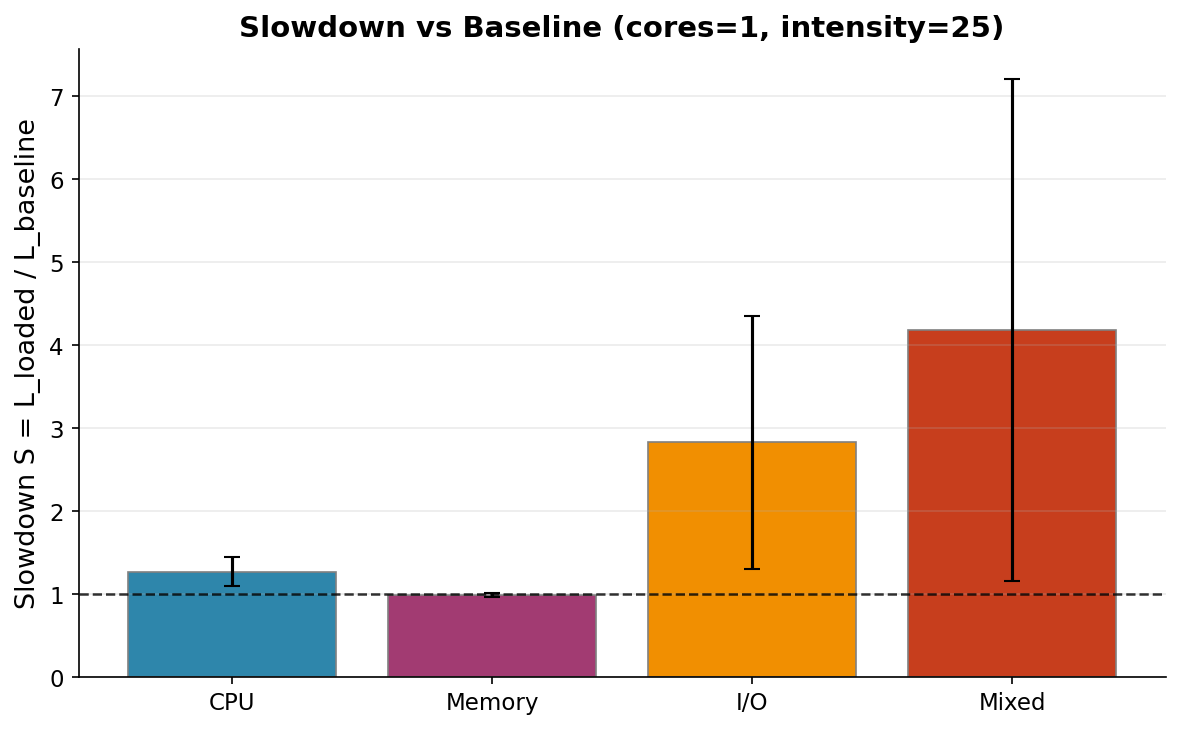
\includegraphics[width=0.98\linewidth]{slowdown_by_workload.png}}
\caption{Normalized slowdown $S$ relative to the single-core, 25\%-intensity
baseline.  Mixed and I/O exhibit the highest degradation.}
\label{fig:slowdown}
\end{figure}

The slowdown plot makes the cross-workload effect easy to see: I/O is already
more than 2.8$\times$ slower than its baseline on average, while mixed
workload exceeds 4$\times$ because it combines the two most contentious paths
in the system.  To see how this changes at the tail rather than only at the
mean, Figures~\ref{fig:tailio} and \ref{fig:tailmixed} show the low and high
percentile behavior for the two most variable workload classes.  Figure~\ref{fig:workcmp}
then compares all workloads side by side at a representative core setting so
the gap between compute-bound and contention-bound behavior is visible in one view.

\begin{figure}[htbp]
\centerline{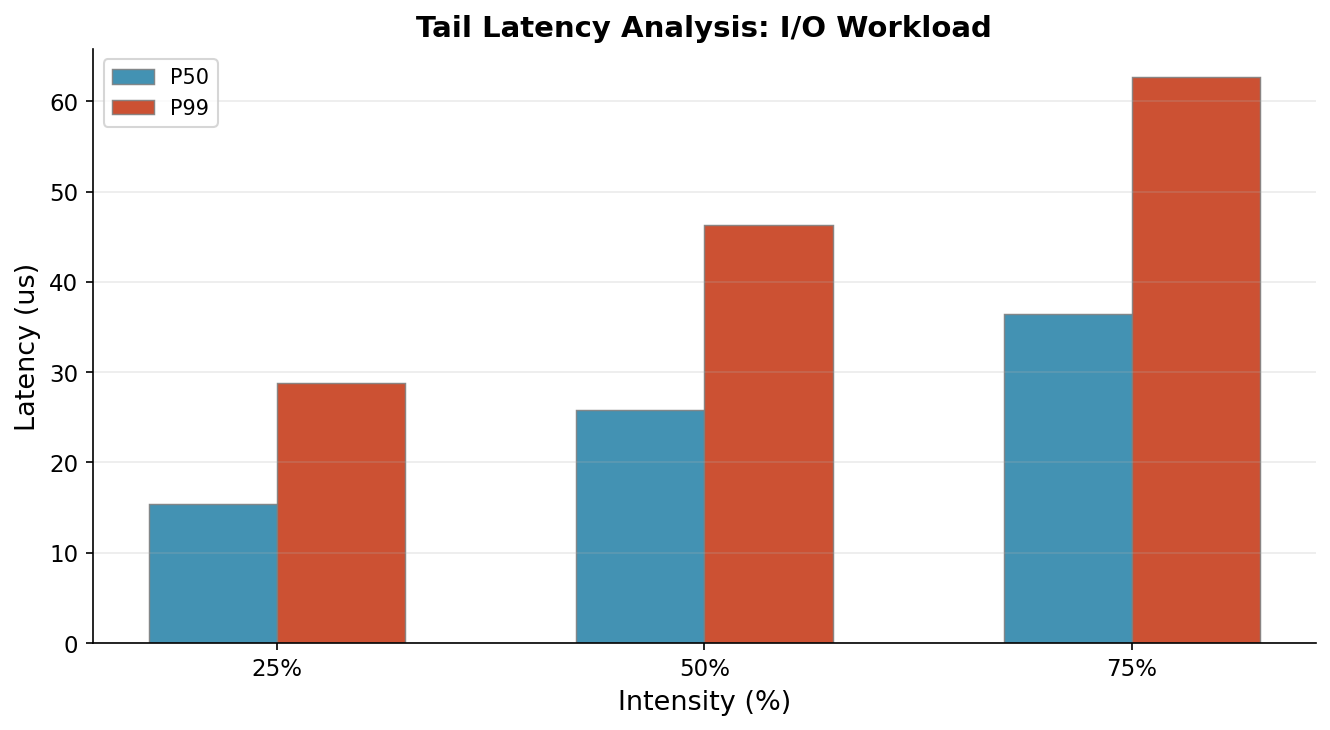
\includegraphics[width=0.90\linewidth]{tail_latency_io.png}}
\caption{P50 and P99 latency for I/O workload by intensity.}
\label{fig:tailio}
\end{figure}

\begin{figure}[htbp]
\centerline{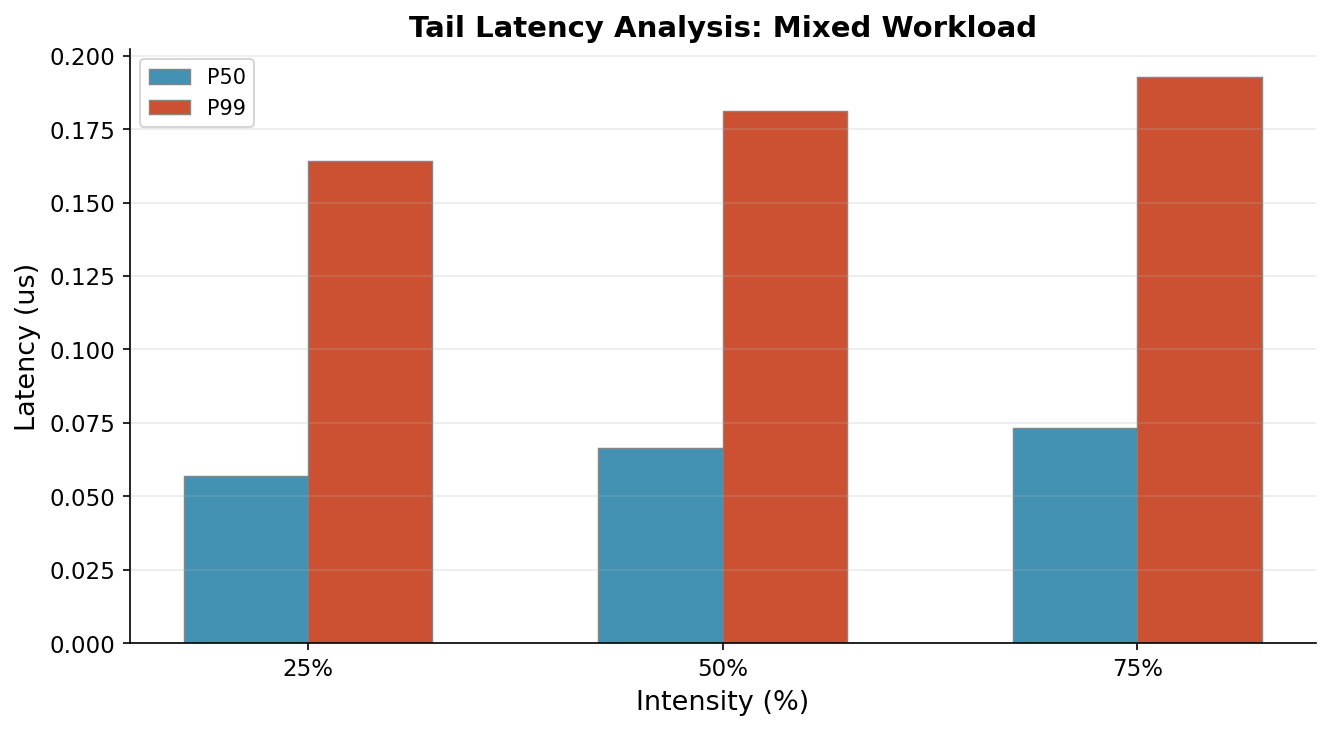
\includegraphics[width=0.90\linewidth]{tail_latency_mixed.png}}
\caption{P50 and P99 latency for mixed workload by intensity.  The large
P50--P99 gap indicates high variability driven by resource contention.}
\label{fig:tailmixed}
\end{figure}

\begin{figure}[htbp]
\centerline{
\includegraphics[width=0.90\linewidth]{workload_comparison.png}}
\caption{Grouped comparison of mean latency across workload types and
intensity levels at a representative core count.}
\label{fig:workcmp}
\end{figure}

%─────────────────────────────────────────────────────────────────────────────
\section{Why Latency Degrades with More Cores}
\label{sec:whyworse}

\subsection{The Root Cause: Shared Resource Contention}

Adding more cores increases total demand placed on shared system resources.
The processor's last-level cache, the memory bus, the kernel run queue, and
the I/O stack are all shared across cores.  When $C$ cores each submit
requests to one of these shared resources, the resource must service $C$ times
as many requests per unit time.  If the resource has finite capacity, requests
queue and each individual request waits longer.

\subsection{Scheduling Overhead}

The Linux scheduler maintains one run queue per CPU core.  Context switches
occur when a process is preempted or when it voluntarily yields the CPU while
waiting for I/O.  Each switch saves and restores the full register file,
updates TLB state, and can invalidate branch predictor history.

Table~\ref{tab:perfmeans} shows 372.7 mean context switches per I/O run and
853.3 per mixed run, far above 45.0 for CPU.  This is because every
\texttt{fsync} call blocks the calling process until the kernel completes the
flush.  At 8 cores, eight processes are concurrently issuing \texttt{fsync}
calls, all competing for the same I/O queue and all generating scheduling
events when they block and wake.

\subsection{Cache Contention}

When multiple cores simultaneously access different memory regions, the
shared LLC must serve all their misses.  If the aggregate working set of all
active workers exceeds LLC capacity, every access that would otherwise be a
cache hit becomes a DRAM access, adding 60--100~ns of latency on this platform.

The cache miss rate for memory workloads (0.52) is already high at one core,
indicating that even the single-worker working set partially exceeds the LLC.
At 8 cores, eight concurrent workers each iterate over their own working set,
multiplying LLC pressure by~8.  This explains the 9\% memory latency rise at
8 cores and the even larger mixed workload degradation, where CPU and memory
threads compete for the same cache space from within the same process set.

The tail-latency plots reinforce the same story but from a different angle.
For I/O, the separation between the median and upper tail widens as intensity
increases, which means that some requests are queued much longer than the
average request.  The mixed workload shows an even larger P50--P99 gap,
which is consistent with a system in which a few unlucky transactions hit a
busy scheduler or cache miss at the wrong time while other transactions still
complete quickly.  In a viva, this is the key distinction to emphasize: the
mean says how the workload behaves on average, while the tail says how bad the
worst cases become for real users.
The results are fully reproducible: the WASP source code, CSV dataset, and
generated figures are co-located and the full sweep can be re-run with a
single shell command on any Linux machine with \texttt{perf\_event\_paranoid}
set to~1.

%─────────────────────────────────────────────────────────────────────────────
\section{Conclusion}
\label{sec:conclusion}

This paper has presented WASP, a framework for understanding how different
categories of workloads respond to increasing core count on a real multicore
processor.  The experimental results from a 240-run evaluation confirm that
the relationship between core count and performance is workload-specific and
is driven by identifiable hardware and OS-level bottlenecks.

I/O workloads suffer most because the storage device and kernel I/O scheduler
become serialization points under concurrent access.  Mixed workloads suffer
from two compounding effects: cache contention from memory threads and
scheduling overhead from blocking patterns.  CPU workloads scale reasonably
but non-linearly on hybrid-core processors.  Memory workloads are the most
stable.

The perf integration in WASP provides counter-based evidence supporting each
of these conclusions, replacing speculation with measurable microarchitectural
data.  The framework is open, reproducible, and extensible to additional
workload types, hardware platforms, and counter sets.

\balance
\bibliographystyle{IEEEtran}
\begin{thebibliography}{00}
\bibitem{gregg2020}
B. Gregg, \emph{Systems Performance: Enterprise and the Cloud}, 2nd~ed.,
Pearson, 2020.

\bibitem{weaver2013}
V. Weaver, ``Linux perf\_event Features and Overhead,''
in \emph{Proc.\ The Linux Foundation Collaboration Summit}, 2013.

\bibitem{lmbench}
L. McVoy and C. Staelin, ``lmbench: Portable Tools for Performance Analysis,''
in \emph{Proc.\ USENIX Annual Technical Conference}, pp.~279--294, 1996.

\bibitem{spec}
Standard Performance Evaluation Corporation, ``SPEC CPU 2017 Benchmark,''
\url{https://www.spec.org/cpu2017/}, 2017.
\end{thebibliography}

\end{document}
